\section{Evaluation}
\label{sec:evaluation}

\begin{itemize}
\item N-fold cross-validation with flat prior, complexity, depth, pcfg or temperley's prior
\item Use different likelihoods: Additive noise, downbeat stretching, louder downbeats
\end{itemize}


We want to know whether a parse got the downbeats right and whether it got the time signature right

If the downbeat is wrong, the upbeat is more likely to be wrong as well (although it may still get the upbeat correct). Getting the downbeats right is the first priority. Level does not matter for downbeats since $(\bullet *)$ does not happen. Level \textit{is} important for upbeats. The second priority is whether is governed by the upbeat slot of the downbeat. The third priority is whether the upbeat is on the right level and with the right division.


We will use n-fold cross-validation to evaluate the parser. To assess the quality of a parse we need some way of measuring how much information about the rhythmic structure was detected correctly by the parser.  Consider a performance with a gold-standard analysis given in figure \ref{fig:eval:a}. The analysis in figure \ref{fig:eval:b} is incorrect, however the parser still correctly identified the relative durations of the units and the quarter notes as downbeats relative to the eighth notes, the only thing that went wrong here is that the first quarter note is identified as an upbeat at the half note level. The analysis in figure \ref{fig:eval:c} also correctly identified the relative durations, but failed to identify the quarter notes as downbeats relative to the eighth note level. While both analysis \ref{fig:eval:b} and \ref{fig:eval:c} are incorrect, analysis \ref{fig:eval:b} more closely resembles the properties of the gold-standard than analysis \ref{fig:eval:c}. This suggests that one criterion of the evaluation should be the extend to which the parser correctly identifies downbeats. 
\begin{figure}
\centering
\subfloat[]{
\label{fig:eval:a}
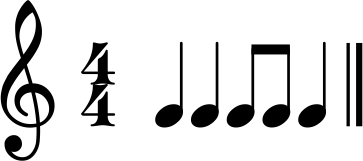
\includegraphics[scale=0.3]{img/eval1}
}
\\
\subfloat[]{
\label{fig:eval:b}
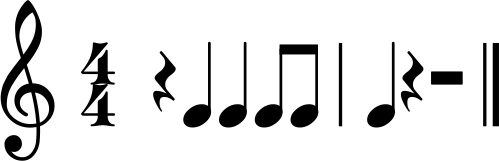
\includegraphics[scale=0.3]{img/eval2}
}
\\
\subfloat[]{
\label{fig:eval:c}
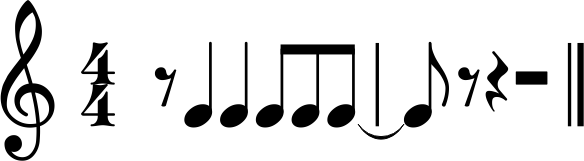
\includegraphics[scale=0.3]{img/eval3}
}
\\
\subfloat[]{
\label{fig:eval:d}
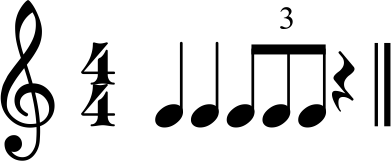
\includegraphics[scale=0.3]{img/eval4}
}
\end{figure}

Another criterion is illustrated by figure \ref{fig:eval:d}, where most of the downbeats were identified correctly but the division of the fourth beat of the measure was identified incorrectly. 

The evaluation that is proposed here incorporates these criteria into two scores
An evaluation is proposed here that incorporates these criteria 
